\section{Turmeric}
\label{sec:turmeric}

\begin{spice}\label{spice:turmeric}
\textsc{Turmeric} \hfill \href{https://powo.science.kew.org/taxon/796451-1}{POWO} \\
\textbf{English:} \textit{turmeric}. 
\textbf{Arabic:} {\arabicfont{كركم}} \textit{kurkum}. 
\textbf{Chinese:} {\tradchinesefont{薑黃}} \textit{jiānghuáng} [ginger-yellow]; 黃薑 \textit{huángjiāng} [yellow-ginger]. 
\textbf{Hungarian:} \textit{kurkuma}.  \\
\noindent{\color{black}\rule[0.5ex]{\linewidth}{.5pt}}
\begin{tabular}{@{}p{0.25\linewidth}@{}p{0.75\linewidth}@{}}
Plant species: & \taxonn{Curcuma longa}{L.} (syn. \taxonn{Curcuma domestica}{Valeton}) \\
Family: & \textit{Zingiberaceae} \\
part used: & rhizome \\
Region of origin: & India \\
Cultivated in: & China; Honduras; India; Indonesia; Jamaica \\
Color: & orange-yellow \\
\end{tabular}
\end{spice}

\begin{figure}[!ht]
	\vspace{-4ex}
	\centering
	\subfloat[]{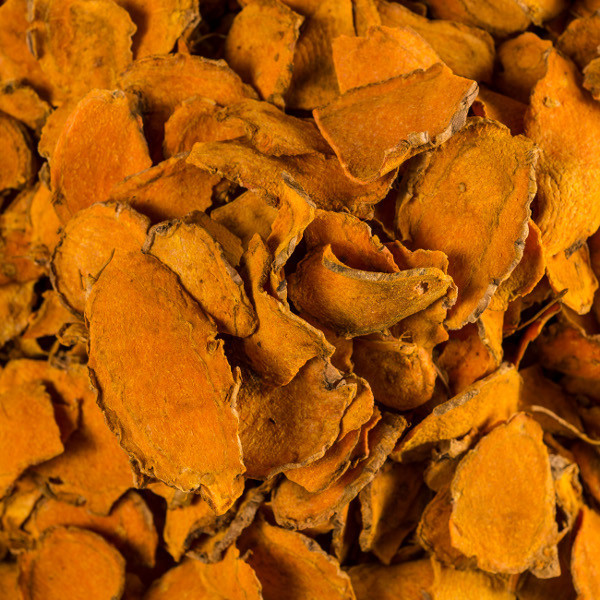
\includegraphics[width=0.3\linewidth]{imgs/spices/turmeric-1.jpg}}
	\hfill
	\subfloat[]{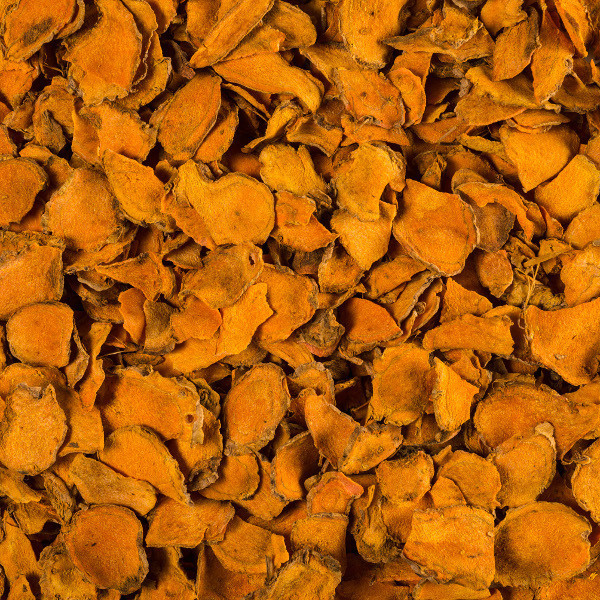
\includegraphics[width=0.3\linewidth]{imgs/spices/turmeric-2.jpg}}
	\hfill
	\subfloat[]{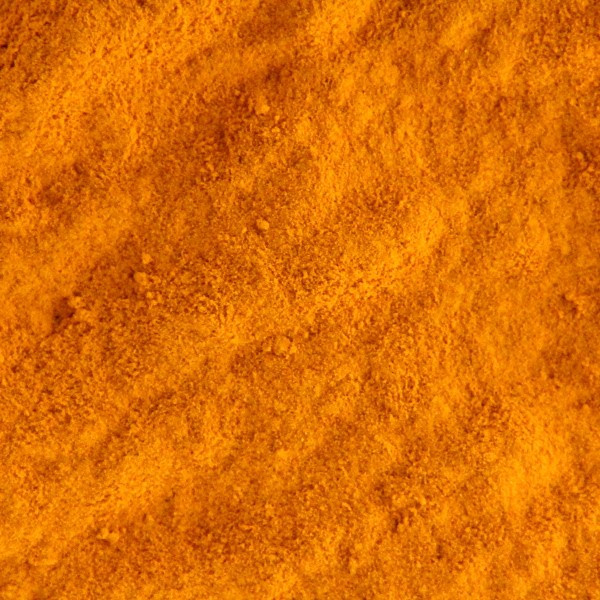
\includegraphics[width=0.3\linewidth]{imgs/spices/turmeric-3.jpg}}
	\caption{vanilla... \taxon{Vanilla planifolia?}. Credits: Aromatiques; Wikimedia Commons (CC4.0)}\footnote{\url{https://commons.wikimedia.org/wiki/File:Saffron_Flowers_in_Khorasan,_Iran.jpg}}
	\label{fig:turmeric_imgs}
\end{figure}

\subsection{The Botany, Origins, and Cultivation of Turmeric}

\subsection{The History of Turmeric}

\subsection{The Names of Turmeric}
\label{sec:names_of_turmeric}

\subsubsection{English}

\begin{etymology}\label{ety:turmeric}
English \textit{turmeric} `turmeric'
< French \textit{terre mérite} `turmeric'
< Medieval Latin \textit{terra merita} `turmeric'\footnote{}
\end{etymology}

\begin{table}[!ht]
\centering
\begin{tabularx}{\textwidth}{@{}l>{\itshape \small}lL>{\small}l@{}}
\toprule
\textbf{\#} & \multicolumn{1}{l}{\textbf{Species}} & \multicolumn{1}{l}{\textbf{Name}} & \multicolumn{1}{l}{\textbf{Source}} \\
\midrule
1	& Curcuma longa	& curcuma	& \textcite{oed} \\
2	& Curcuma longa	& Indian saffron	& \textcite{oed} \\
\textbf{3}	& \textbf{Curcuma longa}	& \textbf{turmeric}	& \textbf{\textcite{van_wyk_culinary_2014}} \\
\bottomrule
\end{tabularx}
\caption{Various names for turmeric in English.}
\label{table:names_turmeric_en}
\end{table}



\subsubsection{Arabic}

\begin{table}[!ht]
\centering
\begin{tabularx}{\textwidth}{@{}l>{\itshape \small}lr>{\itshape}lL>{\small}l@{}}
\toprule
\textbf{\#} & \multicolumn{1}{l}{\textbf{Species}} & \multicolumn{1}{l}{\textbf{Name}} & \multicolumn{1}{l}{\textbf{Tr.}} & \multicolumn{1}{l}{\textbf{Gloss}} & \multicolumn{1}{l}{\textbf{Source}} \\
\midrule
1	& Curcuma longa	& أصابع صفر	& aṣābiʿ ṣufr	& yellow fingers	& \textcite{wikipedia} \\
2	& Curcuma longa	& هرد	& hurd	& 	& \textcite{amar_arabian_2017} \\
\textbf{3}	& \textbf{Curcuma longa}	& \textbf{كركم}	& \textbf{kurkum}	& \textbf{phonetic}	& \textbf{\textcite{amar_arabian_2017}} \\
4	& Curcuma longa	& شجرة الخطاطيف	& shajarat al-khaṭāṭīf	& 	& \textcite{amar_arabian_2017} \\
5	& Curcuma longa	& زعفران هندي	& zaʿfarān hindī	& Indian saffron	& \textcite{amar_arabian_2017} \\
6	& Curcuma longa	& عقدة صفراء	& ʿuqda ṣafrā'	& yellow knob	& \textcite{baalbaki_-mawrid_1995} \\
7	& Curcuma longa	& عروق صفر	& ʿurūq ṣufr	& 	& \textcite{amar_arabian_2017} \\
\bottomrule
\end{tabularx}
\caption{Various names for turmeric in Arabic.}
\label{table:names_turmeric_ar}
\end{table}



\subsubsection{Chinese}

\begin{table}[!ht]
\centering
\begin{tabularx}{\textwidth}{@{}l>{\itshape \small}ll>{\itshape}lL>{\small}l@{}}
\toprule
\textbf{\#} & \multicolumn{1}{l}{\textbf{Species}} & \multicolumn{1}{l}{\textbf{Name}} & \multicolumn{1}{l}{\textbf{Tr.}} & \multicolumn{1}{l}{\textbf{Gloss}} & \multicolumn{1}{l}{\textbf{Source}} \\
\midrule
1	& Curcuma longa	& \tradchinesefont{寶鼎香}	& bǎodǐngxiāng	& treasure-cauldron-spice?	&  \\
2	& Curcuma longa	& \tradchinesefont{黃薑}	& huángjiāng	& yellow-ginger	& \textcite{defrancis_abc_2003} \\
\textbf{3}	& \textbf{Curcuma longa}	& \textbf{\tradchinesefont{薑黃}}	& \textbf{jiānghuáng}	& \textbf{ginger-yellow}	& \textbf{\textcite{kleeman_oxford_2010}} \\
\bottomrule
\end{tabularx}
\caption{Various names for turmeric in Chinese.}
\label{table:names_turmeric_zh}
\end{table}



\subsubsection{Summary}

\begin{table}[!ht]
\centering
\begin{tabularx}{\textwidth}{@{}ll>{\itshape}lLl>{\small}l@{}}
\toprule
\textbf{\#} & \textbf{Language} & \multicolumn{1}{l}{\textbf{Term}} & \textbf{Gloss} & \textbf{Loan} & \multicolumn{1}{l}{\textbf{Source}} \\
\midrule
1	& English	& curcuma	& 	& yes	& \textcite{oed} \\
2	& English	& Indian saffron	& 	& no	& \textcite{oed} \\
3	& English	& turmeric	& 	& yes	& \textcite{oed} \\
\midrule
1	& Arabic	& hurd	& 	& yes	& \textcite{lane_arabic-english_1863} \\
2	& Arabic	& kurkum	& phonetic	& yes	& \textcite{wehr_dictionary_1976} \\
3	& Arabic	& ʿuqda ṣafrā'	& yellow knob	& no	& \textcite{baalbaki_-mawrid_1995} \\
\midrule
1	& Chinese	& huángjiāng	& yellow-ginger	& no	& \textcite{defrancis_abc_2003} \\
2	& Chinese	& jiānghuáng	& ginger-yellow	& no	& \textcite{kleeman_oxford_2010} \\
\bottomrule
\end{tabularx}
\caption{Conventionalized names for turmeric in English, Arabic, and Chinese, found in dictionaries.}
\label{table:names_turmeric}
\end{table}

















% Cantonese: 黃薑 (wong4 goeng1)

% EE:
% (powder made from) the root-stock of the East Indian plant, used in curry powder, etc. XVI. Early forms also tarmaret, tormarith, which appear to be — F. terre mérite, modL. terra merita, of unkn. orig.; the ending shows assim. to -IC.

% OE:
% pungent powder made from the root of an East Indian plant, 1530s, altered from Middle English turmeryte (early 15c.), which is of uncertain origin. "Middle English Compendium" compares Medieval Latin terra merita (16c.), French terre mérite (17c.), literally "worthy earth," though the reason why it would be called this is obscure. Klein suggests it might be a folk-etymology corruption of Arabic kurkum "curcuma, saffron."

% MW:
% modification of Middle French terre merite saffron, from Medieval Latin terra merita, literally, deserving or deserved earth
% First Known Use: 15th century (sense 1a(1))

% AH:
% [Alteration of Middle English termeryte; akin to French terre mérite and New Latin terra merita, turmeric (New Latin, from Latin terra, earth; see ters- in the Appendix of Indo-European roots + merita, feminine past participle of merēre, to deserve; see (s)mer-2 in the Appendix of Indo-European roots).]

% WK:
% From Middle English turmeryte, tarmaret, of uncertain origin. Possibly from Old French terre mérite (“deserving earth”). According to Klein, possibly corrupted from Arabic كُرْكُم (kurkum, “Curcuma”). 